\chapter{成为小魔仙}

\begin{quote}
    羔羊揭开第七印的时候,天上寂静约有二刻……——《圣经·启示录》8:1
\end{quote}

在继续探索\LaTeX 这个庞大且出色的系统前,有必要停下脚步来了解一些重要的概念。实际上,为了成为能在组成这个系统的大量文件中大展身手的“赫尔克里·波洛”\yz{
    Hercule Poirot,阿加莎·克里斯蒂所著系列侦探小说中的主角。
},掌握这些概念是基本的要求。在本章,我们介绍有关计数器、长度、空白和字盒的内容。如果你在使用\LaTeX 时,除了顺从地使用它提供给你的格式外,还想要其他版式,这4个概念会很有用。

\begin{exclamation}
    本章涉及的概念有些微妙的细节,比较难以把握\jz{
        作者本人也不能保证掌握了全部内容……
    }。我们建议你实际上手体验一下,因为这里介绍的工具一方面可以为你生成最令人满意的结果,另一方面也能让你掉最多的头发,基本上跟直接在你头上薅差不多。
\end{exclamation}
\section{计数器}

文档中所有带有编号的对象都由\emph{计数器}生成。计数器可以递增、递减,也可以重设为0,等等。我们也可以根据自己的需要来创建计数器。

\subsection{可用的计数器}

计数器主要与标题、页码、浮动环境(环境\dm{figure}和\dm{table})、方程(环境\dm{equation})、页面底部的注释、编号列表(环境\dm{enumerate})息息相关。

表\ref{tab:4.1}列出了\LaTeX 中基础的计数器的名称。可以注意到,它们基本上都由相关对象的名称组成。计数器\dm{enumi}~\dm{enumiv}分别与环境\dm{enumerate}中的第1层~第4层相关。\dm{mpfootnote}是环境\dm{minipage}中脚注的计数器,会在4.4.3小节提到。

\begin{table}
  \centering
  \ttfamily
  \begin{tabular}{|l|l|l|l|}
    \hline
    part       & paragraph    & figure     & enumi\\
    chapter    & subparagraph & table      & enumii\\
    section    & page         & footnote   & enumiii\\
    subsection & equation     & mpfootnote & enumiv\\
    subsubsection &&&\\
    \hline
  \end{tabular}
  \caption{\LaTeX 的计数器}
  \label{tab:4.1}
\end{table}

\subsection{操作}

在接下来的段落中,我们介绍几个操作计数器的基本工具。注意,计数器是\emph{全局}变量,因此以下描述的三个指令也会在全局范围内生效。同时,也需要注意,其中的变量都是\emph{整数}。

\subsubsection{创建计数器}

可以通过以下指令\emph{创建}计数器:

\begin{dmd}
\backslash newcounter\{\codereplace{计数}\}[\codereplace{父计数}]
\end{dmd}

该指令可以创建一个新的计数器,名为\codereplace{计数}。参数\codereplace{父计数}是非强制的,如果配置,则每次\codereplace{父计数}递增时,\codereplace{计数}都会归零。

\subsubsection{指定计数}

可以通过以下方法为计数器指定一个值:

\begin{dmd}
\backslash setcounter\{\codereplace{计数}\}\{\codereplace{值}\}
\end{dmd}

其中,\codereplace{计数}代表我们想要指定值的计数器,\codereplace{值}即具体指定的值。

\subsubsection{增值}

可以通过以下指令使计数器的值增加或减少:

\begin{dmd}
  \backslash addtocounter\{\codereplace{计数}\}\{\codereplace{值}\}
\end{dmd}

其中,若\codereplace{值}为正数(对应地,负数),则可以使计数器的值增加(对应地,减少)。为了展现该指令的效果,我们在本书的文档中添加以下一行指令:

\begin{dmd}
\verb|\addtocounter{footnote}{357}|
\end{dmd}

\addtocounter{footnote}{357}
可以看到页面下方脚注的编号变化\jz{
  虽然这个值变了这么多属实有些荒谬……
}了。为了接下来的脚注恢复正确的序号,我们在源码中插入以下指令:

\begin{dmd}
  \verb|\addtocounter{footnote}{-357}|
\end{dmd}

\addtocounter{footnote}{-357}
可以看到,现在的脚注序号恢复正常\jz{
  天灵灵,地灵灵!
}了。

\subsection{显示}

使用如下指令可以将计数显示出来:

\begin{dmd}
\backslash the\codereplace{计数器名}
\end{dmd}

实际上,所有可以显示计数器的指令或环境都调用了类似的指令。这样一来,我们有如下指令:

\begin{itemize}
  \item \verb|\thepage|,在此处可以生成“\thepage ”,会在每次换页时调用;
  \item \verb|\thefootnote|,在此处可以生成“\thefootnote ”,会被\verb|\footnote|调用;
  \item \verb|\thesubsection|,在此处可以生成“\thesubsection ”,会被指令\verb|\subsection|调用;
  \item ……
\end{itemize}

“\verb|\the|”家族的指令通常借助以下格式指令定义:

\begin{itemize}
  \item \verb|\arabic{|\codereplace{计数器}\verb|}|;
  \item \verb|\roman{|\codereplace{计数器}\verb|}|和\verb|\Roman{|\codereplace{计数器}\verb|}|;
  \item \verb|\alph{|\codereplace{计数器}\verb|}|和\verb|\Alph{|\codereplace{计数器}\verb|}|。
\end{itemize}

以下是几个示例:

\begin{itemize}
  \item \verb|\arabic{page}|在此处可以生成“\arabic{page}”;
  \item \verb|\alph{footnote}|在此处可以生成“\alph{footnote}”,\verb|\Alph{section}|在此处可以生成“\Alph{section}”;
  \item \verb|\Roman{subsection}|在此处可以生成“\Roman{subsection}”,\verb|\roman{page}|在此处可以生成“\roman{page}”;
  \item ……
\end{itemize}

为了自定义文档,重定义“\verb|\the|”家族的指令的做法很常见。例如,在本书的文档中,指令\verb|\thefigure|以如下形式重定义:

\begin{dmd}
\verb|\arabic{chapter}.\arabic{figure}|
\end{dmd}

这样一来,本书的图题会依次以如下形式编号:

\begin{enumerate}
  \item 阿拉伯数字形式的章号;
  \item 圆点;
  \item 阿拉伯数字形式的图号。
\end{enumerate}

可以以如下的形式重新定义图题编号的显示形式。例如,以如下的形式定义:

\begin{dmd}
\verb|(\Roman{chapter}):\arabic{section}.\arabic{figure}|
\end{dmd}

这样可以在图题中以另一种形式——也是一种相对不整洁的形式——来为图编号。这里,我们重定义了指令\verb|\thefigure|,来生成新的编号方式:先在括号中以罗马数字形式显示章号,再以圆点分隔以阿拉伯数字形式显示的节号和图号。“\textsc{Fig.}”等字样、图号后的连接号等则需要在指令\verb|\caption|的层级去定义。

\begin{figure}[ht]
  \centering
  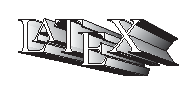
\includegraphics{img/latex.eps}\\
  \textsc{Figure} (IV):1.1: 特殊编号的图题
\end{figure}

\section{长度}

如果说计数器需要依托文档中对象的\emph{序号}而存在,那么长度就定义了实体\emph{占的空间}。长度是\LaTeX 中的一种参数,旨在以某种方式来表述对象的尺寸。

\subsection{单位}

所有的尺寸都需要带有单位。\emph{刚性}\jz{
  我们稍后会看到\emph{弹性}的尺寸。
}的尺寸具有如下形式:

\begin{dmd}
  \codereplace{数字}\codereplace{单位}
\end{dmd}

其中,\codereplace{数字}可以是正值或负值,在需要时也可以带小数;\codereplace{单位}需要是\LaTeX 可以识别的单位。可以使用包括但不仅限于如下列出的单位:

\begin{description}
  \item[cm] \emph{厘米};
  \item[mm] \emph{毫米};
  \item[in] \emph{英寸}(约\dm{2.54cm})\yz{
    目前,1英寸严格定义为2.54 cm,原文中的“约”不严谨。
  };
  \item[pt] \emph{点},通常在排版领域使用,合$\frac{1}{72.27}$英寸;
  \item[em] 当前字体下字母“M”的宽度;
  \item[ex] 当前字体下字母“x”的高度。
\end{description}

注意,单位\dm{em}(对应地,\dm{ex})一般会在水平(对应地,竖直)方向上衡量尺寸时使用,且使我们得以根据当前字体字号来决定尺寸。

\begin{table}[ht]
  \begin{tabular}{lcl}%todo现在是用字母凑的,看看能不能改成真的线段
    \dm{1cm} & : & \textsf{I}\!\rule{1cm}{1pt}\!\textsf{I} \\
    \dm{1in} & : & \textsf{I}\!\rule{1in}{1pt}\!\textsf{I} \\
    \dm{3mm} & : & \textsf{I}\!\rule{3mm}{1pt}\!\textsf{I} \\
    \dm{2em} & : & \textsf{I}\!\rule{2em}{1pt}\!\textsf{I} \\
    \dm{10pt} & : & \textsf{I}\!\rule{10pt}{1pt}\!\textsf{I} \\
  \end{tabular}
\end{table}


\subsection{\LaTeX 中的几个长度}

在\LaTeX 和各个扩展中都存在一些预定义的长度。这些长度一般决定了文档中某个部分的尺寸,例如:

\begin{itemize}
  \item \verb|\parindent|为段首缩进,默认为\dm{15pt};
  \item \verb|\textwidth|和\verb|\textheight|分别定义文本的宽度和高度;
  \item \verb|\baselineskip|定义了相邻两行间的基线距离(本书中为\dm{10pt}\yz{
    本项及下一项的具体尺寸都指原书。
  });
  \item \verb|\parskip|为段间距,初始化为\dm{0pt plus 1pt}\jz{
    关于\texttt{p}\texttt{lus}的含义,参见弹性尺寸部分。%连写plus一词会触发奇怪的编译不过bug
  };
  \item ……
\end{itemize}

需要理解,可以使用这些“内置”长度的函数来表示另一个长度,例如:

\begin{dmd}
\verb|0.5\textwidth|
\end{dmd}

这表示页面文本宽度的一半。再如:

\begin{dmd}
\verb|3\parindent|
\end{dmd}

这表示段间距的三倍。注意,对于长度\verb|-1\baselineskip|,可以直接将其写成\verb|-\baselineskip|。

\subsection{操作长度}

就像计数器,长度也可以使用一些指令来操作。

\subsubsection{创建长度}

以下指令可以创建一个长度:

\begin{dmd}
\backslash newlength\{\codereplace{尺寸}\}
\end{dmd}

其中\codereplace{尺寸}是该长度的名称。长度会被初始化为\dm{0pt}(参见示例4.1)。

\begin{exclamation}
注意,不论指令\verb|\newlength|出现在哪里,它的定义都是\textbf{全局的}。此外,一个长度被定义两次会引发报错。相反,对长度的修改是局部的,只会在它出现的组(\verb|{...}|)内生效。
\end{exclamation}